% Simulating hand-drawn lines with TikZ
% Author: percusse
\documentclass{article}
\usepackage{tikz}
%%%<
\usepackage{verbatim}
%\usepackage[active,tightpage]{preview}
%\PreviewEnvironment{tikzpicture}
%\setlength{\PreviewBorder}{10pt}%
%%%>
\begin{comment}
:Title: Simulating hand-drawn lines with TikZ
:Tags: Decorations;Decorative drawings;Mathematics
:Author: percusse
:Slug: hand-drawn-lines

Sometimes, vector graphics look too clean. This example shows
how to let them appear like hand-drawn with a pencil. It bases
on the "bent" decoration.
\end{comment}
\usetikzlibrary{calc,decorations.pathmorphing,patterns}
\pgfdeclaredecoration{penciline}{initial}{
    \state{initial}[width=+\pgfdecoratedinputsegmentremainingdistance,
    auto corner on length=1mm,]{
        \pgfpathcurveto%
        {% From
            \pgfqpoint{\pgfdecoratedinputsegmentremainingdistance}
                      {\pgfdecorationsegmentamplitude}
        }
        {%  Control 1
        \pgfmathrand
        \pgfpointadd{\pgfqpoint{\pgfdecoratedinputsegmentremainingdistance}{0pt}}
                    {\pgfqpoint{-\pgfdecorationsegmentaspect
                     \pgfdecoratedinputsegmentremainingdistance}%
                               {\pgfmathresult\pgfdecorationsegmentamplitude}
                    }
        }
        {%TO 
        \pgfpointadd{\pgfpointdecoratedinputsegmentlast}{\pgfpoint{1pt}{1pt}}
        }
    }
    \state{final}{}
}
\begin{document}
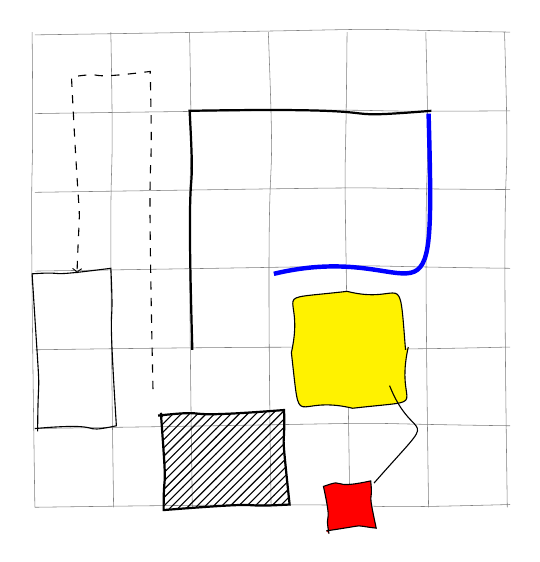
\begin{tikzpicture}[decoration=penciline, decorate]
  \draw[decorate,style=help lines] (-2,-2) grid[step=1cm] (4,4);
  \draw[decorate,thick] (0,0) -- (0,3) -- (3,3);
  \draw[decorate,ultra thick,blue] (3,3) arc (0:-90:2cm);
        % supposed to be an arc
  \draw[decorate,thick,pattern=north east lines] (-0.4cm,-0.8cm)
    rectangle (1.2,-2);
  \node[decorate,draw,inner sep=0.5cm,fill=yellow,circle] (a) at (2,0) {};
        % That's not even an ellipse
  \node[decorate,draw,inner sep=0.3cm,fill=red] (b) at (2,-2) {};
  \draw[decorate] (b) to[in=-45,out=45] (a);
        % This was supposed to be an edge
  \node[decorate,draw,minimum height=2cm,minimum width=1cm] (c) at (-1.5,0) {};
  \draw[decorate,->,dashed] (-0.5cm,-0.5cm) -- (-0.5cm,3.5cm)  -| (c.north);
\end{tikzpicture}
\end{document}